\documentclass[10pt,a4paper]{report}
\usepackage[pdftex]{graphicx}
\usepackage{subfigure}            % Multiple figures per float
\usepackage{placeins}             % Fix float loactions with \FloatBarrier
\usepackage{color}                % Color definitions for boxes
\usepackage{multirow}             % Multiple rows per cell in a table
\usepackage{verbatim}             % Long verbatim sections
\usepackage{titlesec}             % Easy modification the chapter format
\usepackage{fancyhdr}             % Easy modification of header and footer
\usepackage{hyperref}			  % Custom hyperlinks
\usepackage{listings}			  % Code Listings
\usepackage{courier}
\usepackage{graphicx}
\graphicspath{ {images/} }
% inserting images: https://www.sharelatex.com/learn/Inserting_Images

\renewcommand{\arraystretch}{1.0} % Extra space in tables
\parindent0mm                     % New paragraphs start without indentation
\setlength{\parskip}{1em}         % And with a blank line in between

% Redefine chapters to remove the "Chapter" word
\titleformat{\chapter}
  {\normalfont\LARGE\bfseries}{\thechapter}{1em}{}
\titlespacing*{\chapter}{0pt}{3.5ex plus 1ex minus .2ex}{2.3ex plus .2ex}

% Setup hyperlink format in document
\hypersetup{
    colorlinks=true, %set true if you want colored links
    linkcolor=blue,  %choose some color if you want links to stand out
    citecolor=blue,  %choose some color if you want lcitation to stand out
    filecolor=black, % etc...
    urlcolor=blue
}

% Define header and footer
\pagestyle{fancy}
\fancyhf{}
\lhead{Kent Milfeld}
\rhead{amask User Guide}
\lfoot{amask}
\rfoot{\thepage}

% Define header and footer for first page in chapter
\fancypagestyle{plain}{
\fancyhf{}
\lhead{Kent Milfeld}
\rhead{amask User Guide}
\lfoot{amask}
\rfoot{\thepage}
}

% Gray boxes for optional material
\definecolor{LightGrey}{gray}{.85}
\setlength{\fboxrule}{1pt}
\setlength{\fboxsep}{6pt}
\newcommand{\IntroBox}[1]{
  %\fcolorbox[rgb]{0,0,0}{0.95,0.95,0.95}{
    \fcolorbox{black}{LightGrey}{
    \begin{minipage}{0.94\linewidth}
      %\textbf{Introduction}
      #1
    \end{minipage}
  }
}

\lstset{language=C++,
    basicstyle=\ttfamily\scriptsize,
    keywordstyle=\color{blue}\ttfamily,
    stringstyle=\color{red}\ttfamily,
    commentstyle=\color{green}\ttfamily,
    breaklines=true
}

\lstnewenvironment{code}[1][]%
  {\noindent\minipage{\linewidth}\medskip 
   \lstset{basicstyle=\ttfamily\footnotesize,frame=single,#1}}
  {\endminipage}

\lstnewenvironment{smallercode}[1][]%
  {\noindent\minipage{1.1\linewidth}\medskip 
   \lstset{basicstyle=\ttfamily\footnotesize,frame=single,#1}}
  {\endminipage}


\begin{document}

\begin{titlepage}
\thispagestyle{empty}	%don't include number on cover
%\begin{flushleft}
%\begin{figure}
%\includegraphics[width=0.2\textwidth]{gplv3-127x51.png}
%\end{figure}
%\end{flushleft}
\verb+ +
\vspace{1em}
\begin{flushright}
\huge\bf amask v1.0\\
\rule{\textwidth}{4pt}
\large{\bf AMASK: Affinity MASKs for parallel processes/threads\\
Document Revision 1.0\\
\today}
\end{flushright}
\vfill
\begin{figure}[ht!]
       \centering
        
\includegraphics[width=0.5\columnwidth]{images/logo_mask.png}
\end{figure}

%Back of cover page (copyright)
%\newpage
%\thispagestyle{empty}
\vfill
\begin{flushleft}
Kent Milfeld \\
\verb+milfeld@tacc.utexas.edu+\\
\vspace{0.5em}
High Performance Computing \\
Texas Advanced Computing Center\\
The University of Texas at Austin\\
%\vspace{1cm}
\vspace{0.5em}
Copyright 2017 The University of Texas at Austin.
\end{flushleft}
%\newpage
\end{titlepage}

\begin{abstract}

Amask is a set of tools for application developers and users to discover the affinity masks of application
processes (MPI ranks or OpenMP threads) so they can determine where the processes can run.
Amask has the following components:

\begin{itemize}
\item Stand-alone executables to report default masks of OpenMP, 
      MPI or Hybrid executions in an interactive or batch environment.
\item API for instrumenting applications to report affinity masks from within a program.
\item Utilities: timers, set process/thread affinity, create loads (for \verb+top+ viewing)
\end{itemize}


Our intention is to create a tool that provides simple-to-understand affinity
information. Bug reports and feedback on usability and improvements are welcome; 
send to milfeld@tacc.utexas.edu with amask in the subject line. 


If you use amask, cite:

github.com/TACC/amask, ``amask: Affinity Mask'', 
Texas Advanced Computing Center (TACC), Kent F. Milfeld. \cite{amask}

\end{abstract}

\tableofcontents

\chapter{Installation}
Amask is easy to build. Execute \verb+make+  to build the stand-alone executables 
and a library for those who want to instrument their application.

Download the github repository\footnote{\href{https://github.com/TACC/amask}
{https://github.com/TACC/amask}} by clicking on the ``Download ZIP'' file, 
and expanding it in a convenient location.

\begin{verbatim}
    unzip  amask-master.zip
\end{verbatim}

You can also clone the git repository:

\begin{verbatim}
    git clone https://github.com/TACC/amask
\end{verbatim}

This will create a top level directory called \verb+amask+, with subdirectories 
\verb+docs+ and \verb+src+.  Change directory to  \verb+amask+. Edit the \verb+Makefile+ to include an appropriate
MPI compiler and OpenMP flag (the defaults are for Intel).  Execute \verb+make+.

%edit \verb+install.sh+ to reflect your choice for the installation directory. The variables to modify are:

%\begin{table}[h]
%\centering
%\label{tab:env}
%\begin{tabular}{|l|l|l|}
%\hline
%\bf{Variable}	& \bf{Description}                        & \bf{Default}\\\hline
%AMASK\_DIR  & Absolute path to installation directory   & . \\\hline
%\end{tabular}
%\end{table}

%Once these variables are set the tool can be installed by using:

%\begin{verbatim}
%    ./install.sh
%\end{verbatim}

The executables will be placed in the \verb+amask/bin+ directory and the library 
will be placed in \verb+amask/lib+. Include \verb+.../amask/bin+ in your \verb+PATH+ variable.
%unless the \verb+AMASK_DIR=...+ has been modified in the Makefile.

\FloatBarrier
\chapter{Process Thread Affinity Mask for a Parallel Execution}


Execute one of the stand-alone executables, \verb+omp_affinity+, \verb+mpi_affinity+, or
\verb+hybrid_affinity+ in an OpenMP, MPI or hybrid environment, 
respectively, to obtain the expected affinity mask for each 
process/thread for your program in the same environment.  That is,
before you execute your program, execute the appropriate stand-alone affinity
program to get a listing of the masks for each OpenMP thread and/or MPI process
that will occur for your program execution (provided the application doesn't adjust affinity).

In Listing 2.1
a batch job runs the \verb+mpi_affinity+ executable before running an application, to observe
the affinity mask for each rank that the application (\verb+my_mpiapp+) will have.
By removing the \verb+my_mpiapp+ execution line and requesting less time for the batch job, you
can quickly discover the default affinity mask for the parallel environment. 
You can adjust affinity environment variables and quickly assess their impact on 
the affinity masks for your application.  
%If you can acquire an interactive session at your site,
%you can simply adjust the affinity (through KMP\_AFFINITY, OMP\_PLACES, etc.) and run 
%\verb+mpi_affinity+  to make sure your affinity adjustments are doing what you
%think they should do.

\begin{code}[frame=single,breaklines=true,numbers=left,language=C,caption=Listing affinity masks for MPI environment \label{batchamask}]

     #!/bin/bash
     #SLURM  -n 16 -N 1
         ...
     #Batch Script for TACC machine
        ...
      mpirun ./mpi_affinity    #ibrun ./mpi_affinity #@TACC
      mpirun ./my_mpiapp       #ibrun ./my_mpiapp    #@TACC

\end{code}

If a site allows users interactive access to batch nodes (see idev utility @TACC), then
the amask commands can be run interactively. 
Listing 2.2
shows interactive executions to discover the affinity masks
that any pure OpenMP, pure MPI or a hybrid application would have for the environment.
(The environment includes the OMP variables, number of MPI tasks requested, and
MPI affinity environment variables set in the mpi launcher: mpirun, or ibrun at TACC.)

\begin{code}[frame=single,breaklines=true,numbers=left,language=C,caption=Listing OpenMP/MPI and Hybrid masks\label{interactiveamask}]

     export OMP_NUM_THREADS=2; omp_affinity   # pure OpenMP
 
     mpirun -np 4 mpi_affinity                # pure MPI
 
     export OMP_NUM_THREADS=2; mpirun -np 4 hybrid_affinity   # Hybrid

\end{code}
 
% The amask puts a load on the ranks for 10 seconds (default), so that \verb+top+ can be run on
% a node to observe the core occupation. You can change the load time (seconds)
% with the \verb+nsec+ argument on the command line.  In the last command above the MPI processes are
% loaded for 30 seconds.  (Execute \verb+top+, and then press the
% 1 key without hitting the return key, to change the display to show the percentage
% load on each core (or hardware thread when hyperthreading is on).

%%You can reset the load time by setting setting the AMASK\_LOAD\_SECONDS environment
%%variable to a positive integer (units are seconds).

How to read the output:

The output in Listing \ref{amaskdefaultmpienv} is for an 8-rank MPI execution on a 
platform with 2 sockets, 8 cores/socket, no hyperthreading, and processor ids 0-7 
on socket 1 and 8-15 on socket 2.  
One can derive these details from \verb+lstopo+.  
Figure \ref{fig:lstopo1} shows an \verb+lstopo+ report for this system (Sandy Bridge compute 
node on the TACC Stampede machine.)
The same information can be extracted from the contents of the \verb+/proc/cpuinfo+ file.
The \verb+lscpu+ utilitly provides the number of sockets, cores and SMT threads, without
proc-id assignments.

\begin{figure}[t]
\centering
%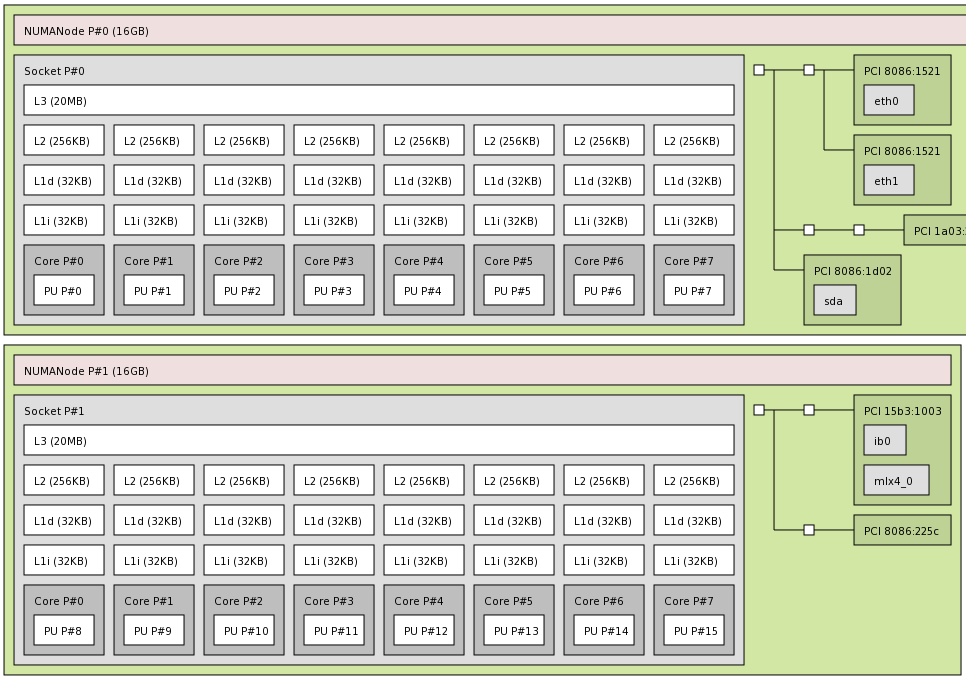
\includegraphics[width=\textwidth]{lstopo}
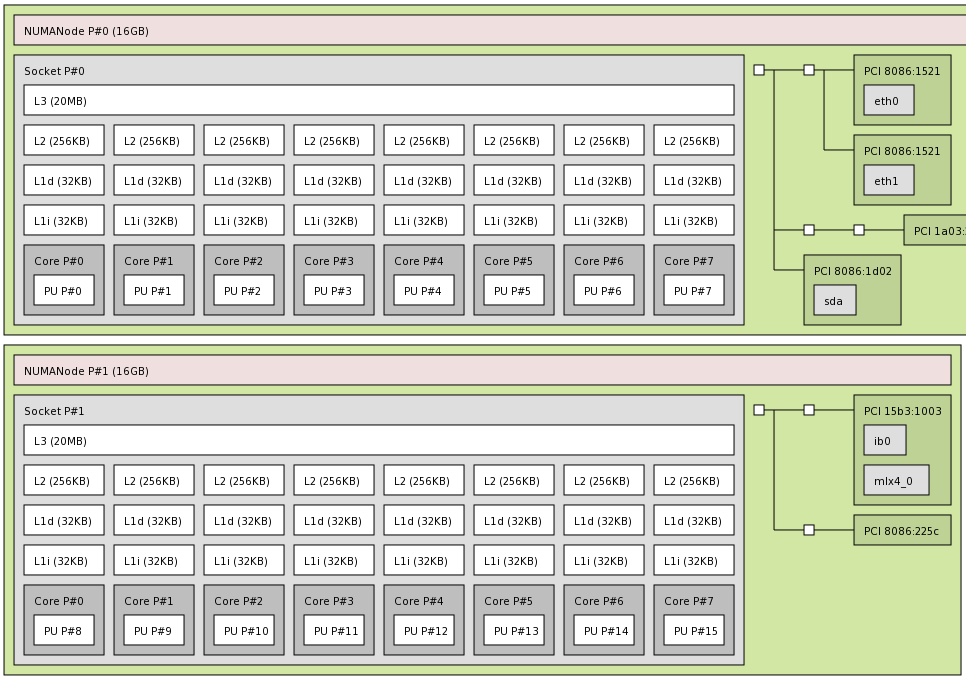
\includegraphics[scale=0.34]{lstopo}
%\caption{Hardware information from lstopo }
\caption{Hardware information from lstopo\label{fig:lstopo1}}
\end{figure}

Listing \ref{fig:lstopo} shows  MPI processes executing on processors (cores) 0-7. 
The rows of the matrix are labeled by the MPI ranks and the columns represent the
machine's processor-ids (\verb+Core P#+ in Figure \ref{fig:lstopo1}) from 0 to Nprocs-1
% where Nprocs is the number \verb+PUs+ from \verb+lstopo+ or the number of processors reported 
% in Figure \verb+/proc/cpuinfo+.  
For this run there are 8 rows, one for each of the 8 MPI ranks (0000 through 0007).
Since there are 16 processors (Nprocs), there are 16 character locations in each row, 
representing the mask bits for processors 0 - 15.
A digit in a row position means that the mask bit is set for the the corresponding
processor, and the MPI process rank listed at the beginning of the row can execute there.
% (for the MPI rank, process, listed at the beginning of the row can execute there). 
When multiple numbers 
are in a row (multiple bits set) it means that the rank can run (float) on any 
of those processors. (The - characters indicate the mask bits are not set.)
The processor id number is determined by adding the digit in the row to the number
directly above in the header. (This quirky approach allows us to represent a 
processor's mask as a set of single characters (digits)
for each bit, and allows one to determine the processor id (proc-id) number by a "look up"-- 
adding the digit in the row to header value above).


\begin{code}[frame=single,breaklines=true,numbers=left,language=C,caption=Default MPI Environment\label{amaskdefaultmpienv}]
$ # 8 tasks requested, MVAPICH2 MPI

$ mpirun mpi_affinity   # non-TACC
$ ibrun  mpi_affinity   # @TACC


      Each row of matrix is an Affinity mask. 
      A set mask bit = matrix digit + column group # in |...|
rank |    0    |   10    |
0000 0---------------   
0001 -1--------------
0002 --2-------------
0003 ---3------------    
0004 ----4-----------   #digit + group # in header = proc-id
0005 -----5----------
0006 ------6---------
0006 -------7--------

\end{code}

The output in Listing \ref{amasktaccenv} is for the same platform as 
\ref{amaskdefaultmpienv}, but the affinity environment has been changed with 
the \verb+tacc_affinity+ script on the ibrun launcher line (\verb+ibrun tacc_affinity mpi_affinity+).
There are other ways to 
change the affinity, such as using another launcher, compiling with 
a different mpi library, or setting MPI environment variables.  In this case 
\verb+tacc_affinity+ positions the first 4 tasks on socket 0, and allows 
each rank to float on any of the processors (cores) of the socket, by setting the first 
8 bits of the mask for each of the 4 ranks, 0-3.  Ranks 4-7
execute on the second socket and are allowed to float across all cores (proc-ids 8-15) 
of the socket.  (\verb+tacc_affinity+ is not part of the amask utilities.)

\begin{code}[frame=single,breaklines=true,numbers=left,language=C,caption=TACC Tailored Environment through tacc-affinity\label{amasktaccenv}]
$ # 8 tasks requested, MVAPICH2 MPI 
$ # + tacc_affinity -- sets MPI affinity @TACC

$ ibrun tacc_affinity mpi_affinity   # @TACC

      Each row of matrix is an Affinity mask. 
      A set mask bit = matrix digit + column group # in |...|
rank |   0     |   10    |
0000 01234567--------       # -- mask to run anyplace on socket1
0001 01234567--------       # rank 1 can execute on any of 0-7 cores
0002 01234567--------       # rank 2 can execute on any of 0-7 cores 
0003 01234567--------       # ...
0004 --------89012345       # -- mask to run anyplace on socket2
0005 --------89012345       # rank 5 can execute on any of cores 8-15
0006 --------89012345       # Bits are for proc-ids (cores) 8,9,10-15  
0007 --------89012345       # Read as 8+0, 9+0, 0+10, 0+10, ... 10+15

\end{code}

A more challenging situation is the determination of the masks on a system with 
hundreds of hardware threads, such as the Intel KNL processor.  At TACC, Stampede2 
has 4,200 PHI 7250 processors (KNLs), each with 272 hardware threads (68 cores x 
4 SMT threads/core).  Before version 1.0  amask would display rows of 272 proc-ids 
(processor ids=hardware threads), but that became a bit unwieldy for users to 
display on laptops.  Now, by default, a matrix of core-ids versus process-ids is displayed.
If there are n SMTs/core, there will be n rows for each process (rank/thread-id) listed (on the left).
For the KNL described above there will be 4 rows displayed for each process 
(corresponding to  proc-id {0-67}, {68-135}, {136-203}, and {204-272}) with the header displaying core-ids.  
This is shown in Listing 2.5.

%\begin{code}[frame=single,breaklines=true,numbers=left,language=C,caption=Process masks for 16 MPI task execution on 68-core KNL\label{amasktaccknl}]

\begin{smallercode}[frame=single,breaklines=true,numbers=left,language=C,caption=Process masks for an 8-thread execution on 68-core KNL\label{amasktaccknl}]

$ export OMP_NUM_THREADS=8
$ export OMP_PROC_BIND=close8
$ ./omp_affinity

      Each row of matrix is an Affinity mask. A set mask bit = matrix digit + column # in |...|
thrd |    0    |   10    |   20    |   30    |   40    |   50    |   60    |
0000 0===================================================================
     --------------------------------------------------------------------
     --------------------------------------------------------------------
     --------------------------------------------------------------------
0001 ====================================================================
     0-------------------------------------------------------------------
     --------------------------------------------------------------------
     --------------------------------------------------------------------
0002 ====================================================================
     --------------------------------------------------------------------
     0-------------------------------------------------------------------
     --------------------------------------------------------------------
0003 ====================================================================
     --------------------------------------------------------------------
     --------------------------------------------------------------------
     0-------------------------------------------------------------------
0004 =1==================================================================
     --------------------------------------------------------------------
     --------------------------------------------------------------------
     --------------------------------------------------------------------
0005 ====================================================================
     -1------------------------------------------------------------------
     --------------------------------------------------------------------
     --------------------------------------------------------------------
0006 ====================================================================
     --------------------------------------------------------------------
     -1------------------------------------------------------------------
     --------------------------------------------------------------------
0007 ====================================================================
     --------------------------------------------------------------------
     --------------------------------------------------------------------
     -1------------------------------------------------------------------

\end{smallercode}

This display is basically core occupation -- something users found they would rather see than 272-character masks.
The proc-id numbers for the 2nd, 3rd and 4th row can be obtained in the usual
manner, but 68, 136, and 204 must be added to the respective row.  
When you need to work directly with the mask and easily determine the proc-ids, it is much easier 
to use the mask display by using the \verb+-ls+ option on command line. 

\FloatBarrier
\chapter{Using the amask Library}

The basic operations used for reporting masks by the \verb+amask+ executables
were collected into a library, so that users
could instrument there own applications to display the masks of MPI processes
and OpenMP threads.

 

\section{Get Masks Inside a Program}

To report the masking from inside a program, include the amask API routine, \verb+omp_report_mask()+,
\verb+mpi_report_mask()+, or \verb+hybrid_report_mask()+, within an OpenMP parallel region, after MPI has been
initialized, or within an OpenMP region of a hybrid program, respectively.  These functions don't
require any arguments or include files:  

\begin{itemize}
\item omp\_report\_mask()
\item mpi\_report\_mask()
\item hybrid\_report\_mask()
\end{itemize}



However, to report masks for hybrid code, it may be necessary
to initialize MPI with the \verb+MPI_Init_thread()+ routine. View the \verb+amask+ codes to see how easy
it is to include them in your own program. The snippets below show how they are to be used:



%\begin{lstlisting}[frame=single,breaklines=true,numbers=left,language=C,caption=Invoking mask report inside code\label{code:apimask}]
\begin{code}[frame=single,breaklines=true,numbers=left,language=C,caption=Invoking mask report inside code\label{code:apimask}]
 // Pure OpenMP code
    #pragma omp parallel
    {
       omp_report_mask();
     ...
    }

 // Pure MPI code
    MPI_Init(NULL,NULL);

       mpi_report_mask();
    ...
    MPI_Finalize();

 // Hybrid code
    MPI_Init_thread(NULL,NULL, MPI_THREAD_MULTIPLE, &provided);

    mpi_report_mask();  // helpful: reports ONLY MPI process masks

   #pragma omp parallel
   {
      hybrid_report_mask();
      ...
   }
   ...
   MPI_Finalize();
\end{code}


\section{Useful Utilities}
\begin{itemize}
\item load\_cpu\_nsec( nsec )   --- Puts load on process/thread for nsec seconds
\item map\_to\_procid(proc-id)   --- Sets process/thread to execute on proc-id
\item gtod\_timer()           --- Easy to use Get Time of Day clock
\item tsc() --- Returns time stamp counter value
\end{itemize}

A thread or process that calls \verb+load_cpu_nsec(int nsec)+ will execute integer
operations (a load) for nsec seconds.  nsec must be zero or a positive integer.  Use the
\verb+cmdln_get_nsec_or_help(int * nsec, int argc, char * argv[])+ function to extract an
integer from the command line for nsec (e.g. \verb+mpi_affinity+ 10).


A thread or process that calls \verb+map_to_procid(int proc-id)+ will assign the
calling thread or process to execute on proc-id, by setting the appropriate
bit in the scheduling mask.  For example, in a parallel region the unique
thread-id returned from \verb+omp_get_thread_num()+ can be used in an
arithmetic operation (linear, modulo, etc.) to create a unique proc-id to be executed on. 

The function \verb+gtod_timer()+ returns a double precision number with the number
of wall-clock seconds since the previous call.  The first call sets the time
to zero. The function uses the Unix \verb+gettimeofday+ utility, and  can be called from 
C/C++ and Fortran.  See comments in the code for
more details.

The function \verb+tsc()+ returns an 8-byte integer (Unix) time stamp count from
the \verb+rdtsc+ instruction. Use this to capture the difference between the counts for
determining 
the cost a of a small set of operations (instructions, code statements). This is
not meant to be used as a general timer, since the processor frequency may change.



\section{Other things you should know}
Build \verb+amask+ with the same MPI library that your 
application will use.  On systems with multi-vendor MPI libraries,
build amap for each vendor version you will use.
With IMPI (Intel MPI) you can set I\_MPI\_DEBUG=4 to
separately report the mask (and other information) for each MPI process. 


\FloatBarrier
\addcontentsline{toc}{section}{\bf References}
\begin{thebibliography}{00}


\bibitem{amask} Amask is a set of executables and routines for reporting affinity information. \href{https://github.com/tacc/amask}{https://github.com/tacc/amask}


\end{thebibliography}

\end{document}
